% !TEX encoding = UTF-8 Unicode

\documentclass[a4paper]{article}

\usepackage{color}
\usepackage{url}
\usepackage[T2A]{fontenc} % enable Cyrillic fonts
\usepackage[utf8]{inputenc} % make weird characters work
\usepackage{graphicx}

\usepackage{enumitem}
\usepackage{bm}
\usepackage{sfmath}
\usepackage{adjustbox}
\usepackage{multirow}

\usepackage[english,serbian]{babel}
%\usepackage[english,serbianc]{babel} %ukljuciti babel sa ovim opcijama, umesto gornjim, ukoliko se koristi cirilica

\usepackage[unicode]{hyperref}
\hypersetup{colorlinks,citecolor=green,filecolor=green,linkcolor=blue,urlcolor=blue}

%\newtheorem{primer}{Пример}[section] %ćirilični primer
\newtheorem{primer}{Primer}[section]
\providecommand{\keywords}[1]{\textbf{\textit{Ključne reči ---}} #1}

\begin{document}

\title{Računarska mreža: Mozak savremenog automobila\\ \small{Seminarski rad u okviru kursa\\Metodologija stručnog i naučnog rada\\ Matematički fakultet}}

\author{Bajić Ana, Krstić Dušica, Stanojević Kristina\\ ana.bajic13@gmail.com, dusica@omikron.org.rs, stanojevic.kristina@gmail.com}
%*********************************ISPRAVITI DATUM, MOŽDA DATUM PREADJE, JER TAD POČINJE DA POSTOJI
\date{18.~april 2018.}
\maketitle

%ENG RECI
%Problem zaustavljanja (eng.~{\em halting problem})

\abstract {U ovom radu je prikazana trenutna arhitektura računarskih mreža u modernim vozilima, sa osvrtom na jedinice za kontrolu rada motora, kontrolu prenosa, kontrolu perifernih delova vozila i kontrole sistema protiv blokiranja kočnica. Zatim su razmatrani različiti protokoli komunikacije između kontrolnih jedinica, a nakon njihovog uvođenja je skrenuta pažnja na ozbiljan nedostatak odbrambenih mehanizama u vozilima. Prikazani su mogući napadi, motivi za njih i jedinice mreže koje su im meta. Na kraju, predstavljeni su već postojeći ali i planirani mehanizmi za odbranu.}

\keywords{CAN, ECU, elektronski moduli, računarska mreža, kontrola vozila, bezbednost mreža}

\setcounter{tocdepth}{1}
\tableofcontents

\newpage

\section{Uvod}
\label{sec:uvod}

Glavna motivacija za razvoj mrežnih tehnologija u vozilima su bili napreci u elektronskoj industriji i nove zakonske regulative koje su postavile znatna ograničenja kako bi se smanjio negativan uticaj automobila na životnu sredinu. Sa striktno postavljenim zahtevima, postalo je nemoguće dostići propisani standard bez pomoći računara. Njihovo korišćenje u ovom domenu su omogućile mreže. Iako mreže nisu bile novo otkriće, njihova primena u automobilskoj industriji jeste. Uspešna implementacija je zahtevala nisku cenu implementacije, stabilnost,  mogućnost funkcionisanja u lošim spoljašnjim uslovima, robusnost i pouzdanost. 

\section{Komponente računarskih mreža}
\label{sec:komponente}

Računarska mreža u vozilu je specijalizovana komunikaciona mreža koja povezuje komponente u vozilu. Glavni preduslovi za postizanje željene kontrole nad vozilom su brzo, "jeftino" i pouzdano razmenjivanje poruka između sistema za kontrolu, nekonfliktnost tih poruka, redundantno rutiranje i otpornost sistema na elektromagnetne smetnje.

U automobilskoj industriji do skorijeg vremena jedini elektronski uređaj u kolima je bio radio, ali danas skoro nijedna komponenata ne može da radi bez neke veze sa računarom - počevši od srca automobila, tj. motora, kako bi se njegove performanse dovele do maksimuma, pa do manje bitnih komponenti kao što je svetlo u kabini.

Od 1996. godine, počevši od Sjedinjenih Američkih Država, svi automobili koji su pušteni u  prodaju moraju imati konektor za kontrolnu dijagnostiku sistema (eng.~{\em On-Board Diagnostics}). OBD daje pristup statusima raznih podsistema u vozilu. Količina informacija, dostupnih kroz ovaj sistem\cite{OBD}, je evoluriala od jednostavnih svetlosnih signala do pružanja standardizovane serije dijagnostičkih kodova problema, što je za rezultat imalo brže identifikovanje i rešavanje problema u vozilu \cite{VB}. 

Glavne komponente računarskih mreža u današnjim vozilima uključuju: 
\begin{enumerate}
	\item Jedinicu za kontrolu rada motora (eng.~{\em Engine Control Unit})\cite{ECU} 
	\item Jedinicu za kontrolu prenosa (eng.~{\em Transmission Control Unit})\cite{TCU} 
	\item Sistem protiv blokiranja kočnica (eng.~{\em Anti-lock Break System})\cite{ABS}
	\item Module za kontrolu perifernih delova vozila (eng.~{\em Body Control Module})\cite{BCM}
\end{enumerate}

Dodavanjem senzora i kombinovanjem informacija, dostupnih kroz ove četiri komponente, mogu se implementirati razni drugi podsistemi u vozilu poput: sistema za regulaciju proklizavanja pogonskih točkova, sistema za sprečavanje blokiranja točkova pri intezivnom kočenju,  sistema za regulaciju dinamike vožnje, elektronska regulacija prenosa snage na pogonske točkove, elektronska regulacija amortizera, sistem za kontrolu proklizavanja itd.

\subsection{Elektronski kontrolni moduli}
\label{subsec:moduli}

Svaki modul predstavlja zaseban čvor na računarskoj mreži, kontroliše određene komponente povezane sa njegovom funkcijom i komunicira sa određenim modulima po potrebi, koristeći standardne protokole za komunikaciju. Mreža kontrolne oblasti (eng.~{\em Control Area Network}), koja predstavlja centralni deo mreže, sadrži prijemnik i odašiljač (eng.~{\em transmitter}) za komunikaciju između sistema za kontrolnu dijagnostiku i kontrolera, kao i za međusobno povezivanje između čvorova.

Kako bi se podržale sve akcije koje su određene nekim konkretnim modulom uz senzore se koriste i aktuatori. Podatke dobijene od senzora (za brzinu, temperaturu, pritisak,  itd.), elektronski kontrolni moduli, koriste dalje u izračunavanjima i dobijene podatke razmenjuju između sebe, kako bi se omogućilo normalno funkcionisanje vozila. Ovo se postiže povezivanjem modula na mrežu. Ovakva arhitektura olakšava posao i proizvođačima jer je moguće dodavati i uklanjati podsisteme bez uticaja na celu arhitekturu \cite{HIW}.

\subsubsection{Jedinica za kontrolu rada motora}
\label{subsubsec:ECU}

Pre pojavljivanja jedinice za kontrolu rada motora, vreme paljenja, idealna brzina i mešavine vazduha i goriva su bili mehanički podešavani i dinamički kontrolisani preko mehaničkih i pneumatskih sredstava. Ova jedinica je tip elektronske kontrolne jedinice koja kontroliše seriju akturatora na sus motoru, kako bi obezbedila otpimalne performanse motora. Ovo se realizuje skupljanjem podataka sa mnoštva senzora koji se nalaze u prostoru motora, interpretacijom tih podataka korišćenjem look-up tabela i prilagođavanjem aktuatora motora u skladu sa obrađenim podacima.

Ukoliko ECU ima kontrolu nad dotokom goriva, onda se naziva jedinica za kontrolu sus motora (eng.~{\em Electronic Engine Management System}). Ceo mehanizam EEMS-a je kontrolisan od strane skupa senzora i aktuatora. 
Posebna kategorija ECU-a su oni koji nemaju fiksno ponašanje i mogu biti reprogamirani od strane korisnika. Oni su potrebni kada se na motoru rade razne izmene nakon proizvodnje. Može se desiti da nakon dodavanja određenih izmena stariji ECU ne podržava novu konfiguraciju, pa se zato priključuje ECU koji se može programirati.

Savremeni ECU koriste mikroprocesor koji omogućava real-time obradu informacija dobijenih od senzora motora. Sastoji se od hardvera i softvera. Hardver je sačinjen od elektronskih komponenti na štampanoj ploči i keramičkog ili tankog laminatnog supstrata. Glavna komponenta na štampanoj ploči je mikro kontrolni čip/centralno procesorska jedinica. Softver je skladišten u mikrokontroloru ili drugim čipovima na štampanoj ploči, obično na EPROM-ovima (eng.{~\em Erasable Programmable Read-Only Memory} \cite{EPROM})ili flash memoriji, tako da se CPU može reprogramirati.

\subsubsection{Jedinica za kontrolu prenosa}
\label{subsubsec:TCU}

Jedinica za kontrolu prenosa je uređaj koji kontroliše moderne elektronske automatske prenose. TCU najčešće koristi senzore u vozilu, ali i podatke koje dobija od jedinice za kontrolu rada motora, da izračuna kako i kada treba promeniti brzinu vozila za optimalne performanse, ekonomičnu potrošnju goriva i pritom da to bude neprimetno putnicima u vozilu.

Dizajn elektronskih automatskih prenosa se menjao od čisto hidromehaničkih kontrola do elektronskih kontrola, koje su u upotrebi od kasnih osamdesetih godina prošlog veka. Do danas, razvoj je bio iterativan i današnji dizajn predstavlja nadogradnju pređašnjih. Aktuatori u menjaču su ključna komponenta u ovim kontrolnim jedinicama.

Evolucija modernog automatskog prenosa i integracija elektronskih kontrola su omogućile ogroman napredak u skorije vreme. Danas je moguće ostvariti bolju potrošnju goriva, smanjeno ispuštanje izduvnih gasova, veću pouzdanost prilikom menjanja brzina, brže i neprimetnije menjanje brzina i bolju kontrolu nad celim vozilom.
U nekim slučajevima se TCU i ECU spajaju u jednu jedinicu - pogonski kontrolni modul.

\subsubsection{Sistem protiv blokade kočnica}
\label{subsubsec:ABS}

Sistem protiv blokade kočnica je bezbednosni sistem koji dozvoljava točkovima na motornom vozilu da zadrže vučni kontakt sa površinom puta u skladu sa kočenjem vozača i sprečava prestanak rotacije točkova i nekontrolisano klizanje po putu. Ovo je automatizovan sistem koji koristi principe ritmičnog kočenja uz menjanje praga kočenja koji postiže mnogo bolju kontrolu i brže kočenje nego što bi većina iskusnih vozača uspela da ostvari.

ABS generalno nudi poboljšanu kontrolu vozila i smanjuje zaustavno rastojanje na suvim i klizavim površinama, iako na površinama pokrivenim šljunkom ili snegom može povećati zaustavno rastojanje i dalje pružati bolju kontrolu nad vozilom. Skorije verzije ovog sistema ne samo da sprečavaju blokiranje točkova nego elektronski kontrolišu i odnos između kočenja prednjih i zadnjih točkova.

Uobičajeno, ABS se sastoji od elektronske kontrolne jedinice (ECU), četiri senzora za brzinu točkova i najmanje dva hidraulička ventila u okviru hidraulike kočnica. ECU konstantno nadgleda rotacionu brzinu svakog točka i u slučaju da se neki točak ne kreće u skladu sa brzinom vozila nego se okreće sporije ili brže, prilagođava ventile kako bi se smanjio ili povećao hidraulički pritisak na kočnice na točkovima, što za rezultat ima smanjenje ili povećanje kočione sile na tom točku pa on počinje da se brže ili sporije okreće.

Moderni ABS sistemi mogu primeniti individualni kočioni pritisak na svaki od četiri točka kroz kontrolni sistem senzora koji se nalazi na glavnini točkova povezanih sa mikrokontrolorom. Često su im dodata dva dodatna senzora, ugaoni senzor na volanu i žiroskopski senzor, koji pomažu sistemu da radi bolje. U slučaju nekog kvara na ABS sistemu, biće signalizirano na kontrolnoj tabli i ABS će biti onemogućen dok se nepopravi. ABS igra glavnu ulogu u podsistemu za zaštitu od proklizavanja vozila.

\subsubsection{Sistem za kontrolu perifernih delova vozila}
\label{subsubsec:BCM}

BCM je elektronska kontrolna jedinica odgovorna za nadgledanje i kontrolu raznih elektronskih dodataka u vozilu, poput: automatskih prozora, retrovizora, klima uređaja, centralnog zaključavanja itd. Komunicira sa drugim sistemima u vozilu preko računarske mreže vozila i njegova glavna primena je da kontroliše aktiviranje releja koji izvršavaju izdate akcije (npr. zaključavanje vrata).

\section{Protokoli komunikacije}
\label{sec:protokoli}

Računarske mreže u vozilima interno povezuju komponente unutar bilo koje vrste vozila. Svi uslovi koji bi trebalo da budu ispunjeni kada se govori o računarskim mrežama, poput sigurnosti u slanju poruka, rešavanje konflikta, minimalno vreme pristizanja poruka, efikasnost i slično, zahtevaju korišćenje protokola posebno definisanih za ovu problematiku. Različiti skupovi ovih modula zahtevaju različite tipove mreže. U dana--šnjim vozilima postoje dva tipa mreže: veoma brze mreže u delu za pogon i spore mreže u sistemu za kontrolu perifernih delova vozila. Podela mreže je takva da predstavlja jednu lokalnu mrežu ili jednu funkcionalnu celinu. U ovim podeljenim mrežama, različiti delovi mreže mogu koristiti različite protokole. Na primer, jedna particija može da koristi CAN protokol, druga LIN protokol itd., kao što je prikazano na slici \ref{fig:protokoliprimer}.

Osnovni zahtevi koje bi trebalo ispuniti jesu efikasno trošenje goriva, eliminisanje bregastih osovina u motoru i delova koji crpe energiju, smanjenje težine vozila, povećanje sigurnosti. U vozilima se često koriste dve serijske magistrale, jedna za sistem koji kontroliše pogon, a druga za periferne delove. Proizvođači se trude da proizvedu što sigurnije vozilo i sa što boljim sistemom za upravljanje vozilom. U tabeli \ref{table:tabela1} se može videti koje protokole koriste neki od proizvođača u zavisnosti od tipa vozila.

\begin{figure}[h]
\centering
 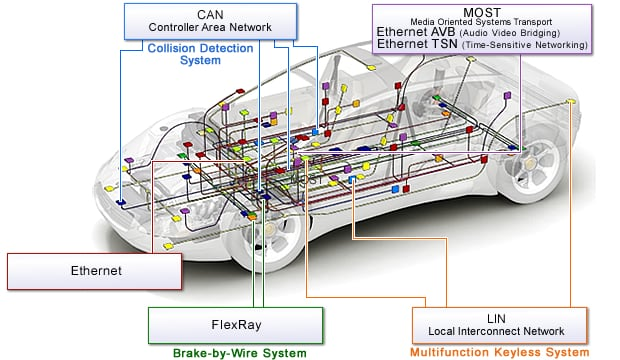
\includegraphics[width=0.9\textwidth]{protokoliprimer}
 \caption{Primer korišćenja protokola u automobilu}
 \label{fig:protokoliprimer}
\end{figure}


Postoje različiti tipovi protokola \cite{viseujednom} koji se mogu koristiti. Neki od tih protokola su:

\begin{itemize}

\item \textbf{CAN} - (eng.~{\em Controller Area Network}) Protokol koji se najčešće koristi kao LAN mreža vozila. Spada u sporu mrežu sa serijskom magistralom za prenos poruka, a koristi Non Return to Zero (NRZ) kodiranje. Sadrži 5 mehanizama za detekciju grešaka.
\item \textbf{FlexRay} - Brza mreža koja omogućava visok stepen fleksibilnosti i pouzdanosti. Koristi point-to-point topologiju zvezde. Magistrala sa ovim protokolom dobro podnosi greške. 
\item \textbf{LIN} - (eng.~{\em Local Interconnect Network}) Koristi se u serijskim magistralama koje služe za komunikaciju između inteligentnih senzora, kao i za periferne uređaje poput klima uređaja, vrata, sedišta i slično. 
\item \textbf{MOST} - (eng.~{\em Media Oriented Systems Transport}) Najčešći protokol kada su u pitanju multimedijalne mreže. Dizajniran tako da omogući prenos audio i video sadržaja kao i podataka visokog kvaliteta. 
\item \textbf{D\textsuperscript{2}B} - (eng.~{\em Domestic Digital Bus}) Multimedijalni interfejs velike brzine. Koristi se u optičkim magistralama koje povezuju audio, video, kompijuterske i telefonske komponente u jednu prstenastu strukturu.  
\item \textbf{Byteflight} - Koristi se u sistemima koji se odnose na sigurnost (na primer za aktiviranje vazdušnog jastuka).
\item \textbf{J1850} - Za deo vozila koji sadrži dijagnostičke aplikacije i aplikacije za deljenje podataka. 
\item \textbf{IEBus} - Protokol zasnovan na CSMA/CD (eng.~{\em Carrier Sense Multiple Access/Collision Detection}) pristupu mreži. Prenos podataka se vrši kroz dve linije, Data+ i Data-, u dva smera. 
\item \textbf{J1708} - Koristi se samo u fizičkom sloju i to u serijskim magistralama, za komunikaciju između mikrokompjutera u vozilu.
\item \textbf{A\textsuperscript{2}B}  - (eng.~{\em Automotive Audio Bus}) Protokol audio distribucije. Ovim protokolom se dobija visoka vernost zvuka (eng.~{\em High fidelity}, Hi-Fi) uz smanjenje težine kablova i veće efikasnosti u trošenju goriva \cite{AB}.  


\end{itemize}



\begin{table}[h!]
\begin{center}
  
\begin{tabular}{ c|c|c|c }
\textbf{Tip protokola} & \textbf{Godina početka} & \textbf{Proizvođač} & \textbf{Tip vozila}\\
\hline
CAN & 1986 & Bosch & razno\\ \hline
\multirow{3}{*}{J1850} & \multirow{2}{*}{-} &  GM & \multirow{12}{*}{automobili} \\
	  & & Ford & \\ \cline{2-3}
             & \multirow{4}{*}{2008} & Chrysler &  \\ \cline{1-1} \cline{3-3}
\multirow{4}{*}{FlexRay}  &    & BMW &  \\
	 		 	 &    & Volkswagen &\\
				 &    & Daimler AG &\\   \cline{2-3}
				 &  - & General Motors &\\ \cline{1-3}
\multirow{4}{*}{MOST} & \multirow{4}{*}{?} & Ford  & \\ 
 &  & BMW & \\ 
 &  & Daimler& \\
 &  &  GM & \\ \cline{1-3}
VAN & 2000 & PSA Peugeot Citroën & \\ \hline
J1708 & 1985 & Volvo AB & teški terenac \\ \hline


\end{tabular}
\caption{Koje protokole koriste neki od proizvođača}
\label{table:tabela1}
\end{center}
\end{table}



\section{Bezbednost mreža}
\label{sec:izazovi}

Svaki računarski sistem može biti preplavljen propustima i slabostima koje napadač može da iskoristi ako je povezan na sistem \cite{6615528}. Elektronskim kontrolnim jedinicama (ECU) nije lako pristupiti van vozila, te implementacija bezbednosnih mehanizama u računarskim mrežama u vozilima nije bila velika briga proizvođača.

%\cite{API}
Umrežavanje je trend današnjice. Moderna vozila često poseduju interfejse koji omogućavaju kako komunikaciju preko magistrala tako i bežičnu komunikaciju. Uvođenjem API-ja (eng.~{\em Application Programming Interface} \cite{API}) za bežičnu komunikaciju, mreže u automobilima su prestale da budu zatvorene i sajber-napadi su postali realnost.

\subsection{Razlozi napada}
\label{subsec:napadrazlog}

Napadači računarskih mreža u automobilima mogu imati jedan ali i više motiva za napad. U nastavku se razmatraju neki od njih, kao i njihove posledice. 

\begin{itemize}
  \item[] \textit{Krađa}
  
  Svakako najočiglednija i najčešća vrsta napada. Napadač može da iskoristi neki prisutni propust u bežičnoj komunikaciji i na taj način tiho i neprimetno otključa automobil i zatim deaktivira alarm.
  \item[] \textit{Elektronska podešavanja}
  
  Napadač je upravo vlasnik ciljanog automobila. Vlasnik može da pristupi kodu ili podacima i promeni ih. Na primer, može da smanji kilometražu automobila pre prodaje, izvrši podešavanje motora i dobije više snage ili instalira nedozvoljene programe. %Takođe, mogu se instalirati jeftine, nelegalne komponente umesto skupljih koje je odobrio proizvođač.
  \item[] \textit{Sabotaža}
  
  % \cite{DOS}
  Sabotaža podrazumeva deaktivaciju ECU, menjanje njihovog softvera ili DOS (eng.~{\em Denial Of Service} \cite{DOS}) napade na mrežu. Posledice ovih napada se protežu od minornih (zaključavanje klima uređaja) do potencijalno smrtonosnih (zaključavanje kočnica). %Ali čak i napadi koji uzrokuju samo male neprijatnosti mogu znatno da utiču na reputaciju proizvođača.
  \item[] \textit{Intelektualna krađa}
  
  Napadač može da pokuša da pristupi poverljivim informacijama o mreži ciljanog vozila. To se može postići prisluškivanjem magistrale ili pristupanjem izvornom kodu neke ECU. Ovakvi napadi mogu da omoguće proizvodnju falsifikovanih ECU. %kao i širenje informacija o propustima u bezbednosti drugim napadačima. 
  \item[] \textit{Povreda privatnosti}
  
  Sa povećanjem broja elektronskih komponenti, povećava se i količina privatnih informacija koje te komponente skupljaju. Napadač može da pristupi telefonskom imeniku vlasnika kao i istoriji poziva ili istoriji GPS koordinata. %ili omiljenim radio frekvencijama. 
%   \item[] \textit{Intelektualni izazovi}
  
%   Mnogi napadači su prosto motivisani izazovom preuzimanja kontrole nad vozilom. Postoje mnogi primeri ovakvih napada kroz istoriju računarstva. 
%   %link ka https://www.cnbc.com/id/100976139
%   %link ka https://en.wikipedia.org/wiki/HackThisSite
\end{itemize}

\subsection{Unutrašnji napadi}
\label{subsec:napadiunutar}

Održavanje bezbednosti mreža je postalo značajan problem s obzirom na to da posledice napada mogu biti veoma ozbiljne, a napadi se mogu lakše izvesti zahvaljujući izuzetno brzom razvoju mreža. Unutrašnji napadi podrazumevaju napade kod kojih napadač ima direktan pristup vozilu. 

\subsubsection{Ranjivost magistrale}
  Ranjivosti koje postoje u trenutnim protokolima, prvenstveno CAN, su detaljno opisane u \cite{security1}, \cite{security2}. Pokazano je da CAN ne može da garantuje sledeće osobine:
  \begin{itemize}
  	\item Poverljivost: 
    
    Dizajn je takav da se svaka poruka poslata na CAN i fizički i logički šalje svakom čvoru. Ovo omogućava zlonamernim čvorovima da prisluškuju magistralu i čitaju sadržaj svakog paketa.
    \item Autentifikacija:
    
    CAN paket ne podrazumeva polje za autentifikaciju svog pošiljaoca. Dakle, svaki čvor može da pošalje poruku koju bi trebalo da može da šalje samo jedan specifičan čvor.
    
    \item Dostupnost:
    
    Veoma je lako izazvati DOS napad na magistrali. Na primer, neka jedinica može da preplavi magistralu paketima visokog prioriteta i time zaustavi prenos paketa ostalih ECU.
    \item Integritet:
    
    %\cite{CRC}
    CAN koristi CRC (eng.~{\em Cyclic Redundancy Check} \cite{CRC}) da proveri da li je poruka promenjena usled greške. Ovaj mehanizam ne može da spreči napadača koji želi da promeni ispravnu poruku jer je lako napraviti ispravan CRC za lažnu poruku.     
  \end{itemize}

\subsubsection{Lokalni napadi}
\label{subsubsec: loknap}  
  Napadi na magistralu se mogu izvršiti ili povezivanjem uređaja na magistralu ili preko OBD (eng.~{\em On Board Diagnostics}) porta. OBD predstavlja sposobnost vozila da identifikuje i prijavi postojeće probleme. Preko ovog porta se može prisluškivati komunikacija na magistrali ali mogu se slati i paketi.

%validan izvor instrukcija \cite{security3}
  Postoje mnogi dokumentovani primeri napada bazirani na direktnom pristupu unutrašnjoj mreži. Napad počinje iz 'black-box' perspektive \cite{security2}. Na taj način, napadač se upoznaje sa značenjem paketa i njihovih identifikatora. Zatim, zlonamerna ECU može da ponovi kontrolne instrukcije i pošalje ih drugim ECU, predstavljajući se kao validan izvor instrukcija \cite{security3}. Neke ECU je čak moguće i reprogramirati kroz mrežu \cite{5504804}, čime se vozilo ostavlja u kompromitovanom stanju.
  
  Koscher u svom radu \cite{5504804} prikazuje način napada na ECU koja se nalazi na delu magistrale koji se razlikuje od ulazne tačke napadača. Napad se može izvršiti tako što se prvo ciljaju i reprogramiraju ECU koje predstavljaju kapiju između magistrala. %, tako da one ECU koje se nalaze na delu magistrale male brzine mogu da šalju poruke ECU na brzim delovima magistrale, čija je bezbednost kritična. 
  
  Dakle, ako napadač kontroliše makar jedan čvor mreže, trenutna arhitektura i protokoli su takvi da mu je omogućeno da preuzme kontrolu nad bilo kojom ECU vozila. Mogao bi se postaviti argument da je potreban direktan, fizički pristup kako bi se izvršio bilo koji od navedenih napada. Sa druge strane, moderni automobili poseduju mogućnost bežične komunikacije. Napadačima više nije potreban direktan pristup ciljanom vozilu. U sledećem odeljku će biti prikazani takvi napadi.
  %Dakle, napadač bi prvo morao da ima pristup vozilu a zatim da ugradi uređaj u magistralu. U većini slučajeva, brže i lakše bi bilo napasti vozilo ne-elektronski (npr. lakše je iseći kočnice nego napasti odgovarajući ECU). 

\subsection{Spoljašnji napadi}
\label{subsec:napadispolja}

2011. godine, Checkoway je uspeo da reprodukuje napade opisane u prethodnom odeljku pronašavši i iskoristivši ranjivosti u interfejsu za komunikaciju, bez fizičkog pristupa samoj mreži \cite{5504804}. Spoljašnji napadi mogu biti grupisani na sledeći način, po distanci: indirektan pristup, bežični pristup malog dometa i bežični pristup širokog dometa. Svaki od ovih pristupa će u nastavku biti opisan i biće dati neki mogući scenariji napada.

\subsubsection{Indirektan pristup}  
\label{subsubsec:napadiindirekt}

  U ovom odeljku, pažnja je posvećena napadima koji se oslanjaju na kompromitovanim uređajima koji će biti povezani sa vozilom. Za razliku od unutrašnjih napada, povezivanje sa mrežom ne čini napadač, već vlasnik vozila.

\begin{itemize}
  	\item OBD port:
    
    Ranije (odeljak \ref{subsubsec: loknap}) je prikazano kako se sam OBD port može koristiti u napadima. U ovom slučaju, meta napada je uređaj za dijagnostiku koji je priključen na port. Taj uređaj se kontroliše putem laptopa preko WiFi-a: ranjivosti u API-u za komunikaciju su omogućile da se ubaci shell skripta u taj uređaj preko drugog laptopa na istoj WiFi mreži. Zatim bi uređaj emitovao zlonamerne pakete preko mreže vozila svaki put kad bi bio priključen \cite{Checkoway}.
    
	\item CD plejer:
    
    U radu \cite{Checkoway} su identifikovane dve ranjivosti u CD plejeru. Ubacivanje CD-a na kome se nalazi datoteka specifičnog imena može da zavara plejer da pomisli da je u pitanju neko fabričko ažuriranje. Uređaj će zatim instalirati novi, maliciozni softver. Još jedan propust je u dekodovanju audio datoteka - moguće je napraviti datoteku koja će izazvati slanje poruka preko magistrale dok je plejer čita.

%     \item USB port:
    
%     Jedan od mogućih slučajeva je sličan prethodnom - muzički uređaj vozila može da pročita malicioznu datoteku sa fleš memorije. Moguć je i slučaj gde je kompromitovan uređaj (pametni telefon ili mp3 plejer) povezan sa vozilom, koji bi zatim izvršio napad na ECU na koju je povezan.

  \end{itemize}
  
\subsubsection{Napadi malog dometa}
\label{subsubsec:napadimalo}

Ovi napadi koriste bežične komunikacione tehnologije. Mogu biti direktni, gde se napada komunikacioni modul vozila, i indirektni, gde se napada uređaj vozača koji se može priključiti na vozilo.
  \begin{itemize}
  	\item Bežično povezivanje sa mobilnim uređajem:
    
    Savremena vozila je moguće spojiti sa različitim uređajima putem Bluetooth konekcije. Implementacije ovakvih protokola mogu imati propuste. Ti propusti se mogu iskoristiti za osluškivanje konverzacija, prikupljanje podataka kao i samo kompromitovanje ECU \cite{Checkoway}.

    \item Komunikacija između vozila:
    
    Komunikacija između vozila je u razvoju. Vozilo će moći da komunicira sa drugim vozilima na putu tako što će ih obaveštavati o svom statusu. Na primer, vozilo će moći da obavesti svog vozača o mogućoj nesreći (ako vozilo ispred naglo zakoči ili ako ima nadolazećih vozila na raskrsnici) ili će moći samo da se prilagodi novonastalim uslovima. Analizom rizika došlo se do zaključaka da se komunikacija između vozila može prisluškiavti, mogu se slati lažni podaci kako bi se izazvale neprikladne rekacije vozila kao i da se mogu kompromitovati ECU odgovorne za ovu komunikaciju \cite{6463997}.
  \end{itemize}

\subsubsection{Napadi širokog dometa}
\label{subsubsec: napadisiroko}

U ovu kategoriju spadaju napadi koji se prenose preko bežičnih komunikacionih tehnologija dalekog dometa. Potreban je kanal za prenos dugih signala kao i kompromitovanje uređaja posrednika.

  \begin{itemize}
  	\item Mobilna telefonija:
    
    Checkoway je otkrio nekoliko ranjivosti u uređaju za telekomunikaciju \cite{Checkoway}. Iskoristivši to, uspeo je da izvrši proizvoljan kod koji je preuzeo putem 3G mreže i time kompromituje vozilo.
    
    \item Aplikacije:
    
    Slično trendu koji je prisutan na pametnim telefonima, neki proizvo--đači vozila nude aplikacije koje je moguće preuzeti sa njihovih web prodavnica. Uspešan napad na samu prodavnicu, ili pak postavljanje programa koji sadrži virus bi mogao da ima veoma ozbiljne posledice na mrežu vozila.
  \end{itemize}


\subsection{Mehanizmi zaštite}
\label{subsec:mehanizmi}

Vozila poseduju mnoge komunikacione kanale koji lako mogu postati ulazne tačke u mrežu za napadače. Što je više napada, i što su oni napredniji, to se više kontramera sprovodi. U ovom odeljku su predstavljene tehnike zaštite koje su trenutno u razvoju.

Postoji veliki broj odbrambenih mehanizama za slične napade na regularne računare. Za razliku od njih, računari u vozilima imaju neka ograničenja. Najveće ograničenje predstavlja hardver \cite{Wolf2007}. Računari u vozilima poseduju malu, ograničenu memoriju i snagu, te ECU ne mogu da izvršavaju napredne kriptografske funkcije kojima se postiže jaka enkripcija. Takođe, za izvođenje kompleksnih instrukcija je potrebno više vremena, a potrebno je da aplikacije rade brzo kako bi se osigurala bezbednost vozila i putnika. Dakle, bezbednosni mehanizmi ne smeju previše uticati na performanse softvera.    

Hardver mora biti proizveden tako da dugo traje i bude izdržljiv (neke komponente moraju da izdrže visoke temperature, pritisak itd.). Softver za zaštitu bi trebalo proizvesti tako da ga je lako ažurirati. Nije lako ni jeftino, a čak ni moguće, zameniti i unaprediti hardver na kome se nalazi softver za zaštitu.  

%Tokom vožnje, pažnja vozača je usmerena na put. Mehanizmi za zaštitu moraju posedovati visok stepen autonomnosti, a intervenciju vozača moraju tražiti samo u ekstremnim situacijama.

\subsubsection{Zaštita spoljašnje komunikacije}
\label{subsubsec: spoljkom}

Kao što je prikazano u prethodnom odeljku \ref{subsubsec: loknap}, jedan propust u rukovođenju komunikacijama je dovoljan da se kompromituje celo vozilo. Prvi korak je zaštita tih kanala. Mnogi od navedenih napada su bili mogući zbog mana u implementaciji samog softvera ili neslaganja sa specifikacijama proizvođača. Neki od njih su mogli biti sprečeni striktnim pridržavanjem dobrih programerskih praksi i postojećih preporuka o komunikacionim protokolima \cite{Padgette}.

Sa druge strane, postoji mnogo različitih proizvođača koji imaju razli--čite standarde, te je nemoguće napisati softver koji je saglasan sa svim preporukama i specifikacijama. Proizvođači vozila su postali svesni ovih problema i počeli su da finansiraju velike projekte. Neki od njih, na primer SEVECOM \cite{SEVECOM}, PRESERVE \cite{PRESERVE} i EVITA \cite{EVITA}, imaju za cilj dizajniranje bezbednih arhitektura za komunikaciju unutar i između vozila.

\subsubsection{Unutrašnja zaštita}
\label{subsubsec: unutkom}

Trenutno se razmatra više rešenja kad je u pitanju bezbednost CAN magistrale. Možemo ih grupisati u tri kategorije: kriptografska rešenja za autentifikaciju i enkripciju paketa koji se šalju preko magistrale, rešenja za detekciju anomalija koje se javljaju u sistemu i rešenja koja osiguravaju integritet softvera.

\begin{itemize}

	\item Kriptografija

	%Kao što je ranije prikazano, bilo koja poruka koja ja poslata preko CAN magistrale se šalje svim čvorovima vezanim za nju. Takođe, ne postoji način autentikacije pošaljioca poruke. 
    %ispravan ključ mogu pročitati \cite{LibraCan}
    Kriptografska rešenja omogućuju autentifikaciju ECU, provere integriteta i enkripcju poslatih paketa, čime ga samo čvorovi koji poseduju ispravan ključ mogu pročitati. Kako kriptografski algoritmi ne bi ometali izvršavanje ostalih funkcija sistema, mogu se koristiti hardverski moduli koji isključivo služe za izvršavanje kriptografskih operacija. 

	\item Detekcija anomalija

	Prate se podaci koji se prenose između ECU i potvrđuje se njihova ispravnost. Na primer, prati se razmak između dva poslata paketa i, ako je on prekratak, ECU koji ih je poslao se blokira. Drugo rešenje je da se svakom paketu dodeli poseban identifikator koji predstavlja ECU koji može da ga šalje. Time je obezbeđeno da taj paket može poslati samo jedna ECU. 

	\item Integritet ECU softvera
    
    Preduzimaju se mere koje štite kritični softver vozila. Na primer, EVITA definiše pouzdanu platformu vozila, čime se štiti ECU namenjen multimediji. Ovime se razdvaja kritični softver (koji može da šalje pakete preko magistrale) od potencijalno nepouzdanih modula. Ti moduli se postavljaju u posebne virtualne mašine, koje su odvojene od kritičnih delova mreže. 
\end{itemize}

\section{Zaključak}
\label{sec:kraj}

Komunikacione mreže se brzo razvijaju i novi tipovi su neophodni na tržištu zbog novih ideja klijenata, zadovoljavanja zahteva bezbednosti i postizanja optimalnih performansi. Sledeće što se u budućnosti očekuje jeste povezivanje komponenti preko interneta, upravo zato što količina podataka koju treba prenositi vremenom raste. U vozila će se ubaciti sistemi zasnovani na Ethernet-u. Svaka komponenta vozila će imati svoju IP adresu, tako da centralizovani računar i ruter u vozilu mogu da šalju i usmeravaju velike količine podataka brzo i efikasno. U razvoju su i automatizovana, samovozeća vozila, koja predstavljaju budućnost automobilske industrije. Zbog velikih troškova ali i zbog povećane pažnje posvećene kvalitetu bezbednosti, napredak na ovom polju je spor, ali neminovan.  

\section{Zahvalnice}

Zahvaljujemo se kolegi Momirov Đorđu na sugestijama i prevodima na srpski jezik i kolegi Nemec Miodragu na recenziranju rada i pruženim konstruktivnim kritikama. Takođe se zahvaljujemo svim anonimnim recezentima koji su doprineli kvalitetu rada. 

\addcontentsline{toc}{section}{Literatura}
\appendix
\bibliography{seminarski} 
\bibliographystyle{plain}



\end{document}
